\documentclass[10pt]{article}
\usepackage[margin=1.4in]{geometry}

% Basic
\usepackage[utf8]{inputenc}
% \usepackage[spanish,mexico]{babel}

\usepackage{parskip}
\usepackage{float}
\usepackage[svgnames]{xcolor}
\usepackage{listings}

\lstset{language=R,
    basicstyle=\small\ttfamily,
    stringstyle=\color{DarkGreen},
    otherkeywords={0,1,2,3,4,5,6,7,8,9},
    morekeywords={TRUE,FALSE},
    deletekeywords={data,frame,length,as,character},
    keywordstyle=\color{blue},
    commentstyle=\color{DarkGreen},
}
\lstdefinestyle{myCustomMatlabStyle}{
  language=Matlab,
  numbers=left,
  stepnumber=1,
  numbersep=10pt,
  tabsize=4,
  showspaces=false,
  showstringspaces=false
}

% Custom colors
\usepackage{color}
\definecolor{deepblue}{rgb}{0,0,0.5}
\definecolor{deepred}{rgb}{0.6,0,0}
\definecolor{deepgreen}{rgb}{0,0.5,0}

% Default fixed font does not support bold face
\DeclareFixedFont{\ttb}{T1}{txtt}{bx}{n}{10} % for bold
\DeclareFixedFont{\ttm}{T1}{txtt}{m}{n}{10}  % for normal

% Python style for highlighting
\newcommand\pythonstyle{\lstset{
language=Python,
basicstyle=\ttm,
otherkeywords={self},             % Add keywords here
keywordstyle=\ttb\color{deepgreen},
emph={MyClass,__init__},          % Custom highlighting
emphstyle=\ttb\color{deepred},    % Custom highlighting style
stringstyle=\color{deepgreen},
frame=tb,                         % Any extra options here
showstringspaces=false            %
}}
% Python environment
\lstnewenvironment{python}[1][]
{
\pythonstyle
\lstset{#1}
}{}


\usepackage{booktabs}
\usepackage{hyperref}
\usepackage{csquotes}
\usepackage{enumitem}

% Math stuff
\usepackage{amsmath, amsfonts, mathtools, amsthm, amssymb}
\usepackage{gensymb}
\usepackage{siunitx}



% Headers
\usepackage{fancyhdr}
\usepackage{lastpage}
\pagestyle{fancy}
\setlength{\headheight}{40pt}

% Commands
\newcommand\N{\ensuremath{\mathbb{N}}}
\newcommand\R{\ensuremath{\mathbb{R}}}
\newcommand\Z{\ensuremath{\mathbb{Z}}}
\newcommand\Q{\ensuremath{\mathbb{Q}}}
\newcommand\C{\ensuremath{\mathbb{C}}}

%Images
\usepackage{import}
\usepackage{xifthen}
\usepackage{pdfpages}
\usepackage{transparent}

\newcommand{\incfig}[1]{%
    \def\svgwidth{\columnwidth}
    \scalebox{.75}{\import{./figures/}{#1.pdf_tex}}
}

\title{Descomposición en valores singulares}
\author{Sergio Arnaud Gómez}
\date{30 de octubre del 2017}

\newtheorem{teo}{Teorema}
\newtheorem{lema}{Lemma}

\newenvironment{solution}
  {\renewcommand\qedsymbol{$\blacksquare$}
  \begin{proof}[Proof]}
  {\end{proof}}
\renewcommand\qedsymbol{$\blacksquare$}


\begin{document}

\lhead{Sergio Arnaud}
\rhead{ Statistical learning (MT7038) \\ Proyect 3 - Neural networks }
\cfoot{\thepage of \pageref{LastPage}}

\section{Backpropagation}

The purpose of this assignment is to implement a complete solution for training a neural network. In practice this is of course done by packages and programs, but it is important to have done it at least once yourselves.

Using backpropagation and stochastic gradient descent we will fit a nerual network with two hidden layers, and sigmoid activation, to the function $y(x) = x^3$ on the interval $(-2, 2)$. Let $\theta = \{(W_i, b_i), i = 1, 2, 3\}$ be the parameters of the model, then the network function is given by

\begin{align*}
    f(x,\theta) = W_3h_2 + b_3 \quad h_2 = \sigma(W_2h_1 + b_2) \quad h_1 = \sigma(W_1x + b_1)
\end{align*}

\subsection{Dimensions of the Parameters}

Assume that both hidden layers has $n$ hidden units, i.e. $h = (h1, . . . , hn)$ . Give the dimensions of all the
parameters $(W_i,bi)$, $i=1,2,3$
\begin{align*}
    W_1 \in \mathbb{R}^{n \times 1} \quad b_1 \in \mathbb{R}^{n \times 1}\\
    W_2 \in \mathbb{R}^{n \times n} \quad b_2 \in \mathbb{R}^{n \times 1} \\
    W_3 \in \mathbb{R}^{1 \times n} \quad b_3 \in \mathbb{R} \ \ \ \ \
\end{align*}

\subsection{Calculating the Derivatives.}

Let $L(x_i, y_i, \theta) = (y_i - f(x_i; \theta))^2$. Given the observation $(x,y)$ calculate the derivatives of $L(x,y;\theta)$.

\begin{align*}
    \frac{\partial L}{\partial W_{i}^3} &= 2(y-f(x,\theta))h^2_i\\
    \frac{\partial L}{\partial b_{i}^3} &= 2(y-f(x,\theta))\\
    \frac{\partial L}{\partial h_{i}^2} &= \frac{\partial L}{\partial b_{i}^3}W_i^3 \\\\
    \frac{\partial L}{\partial W_{ij}^2} &= \frac{\partial L}{\partial h_{i}^2}(h_i^2(1-h_i2))h_j^1 \\
    \frac{\partial L}{\partial b_{i}^2} &=  \frac{\partial L}{\partial h_{i}^2}(h_i^2(1-h_i2)) \\
    \frac{\partial L}{\partial h_{i}^1} &= \frac{\partial L}{\partial b_{i}^2}W_{ii}^2 \\\\
    \frac{\partial L}{\partial W_{i}^3} &= \frac{\partial L}{\partial h_{i}^1}(h_i^1(1-h_i^1))x \\
    \frac{\partial L}{\partial b_{i}^3} &= \frac{\partial L}{\partial h_{i}^1}(h_i^1(1-h_i^1)) \\
\end{align*}

\subsection{Fitting the Model}

The following code fites a feed forward neural network with 2 hiddel layers (125 hidden units) to the function $y(x) = x^3$.

\begin{lstlisting}[language=R]

sigm <- function(x){
  f <- function(y){
    return(1/(1+exp(-y)))
  }
  return( sapply(x,f) )
}

initParams <- function(nrHiddenUnits, xDim) {
  W <- list()
  b <- list()

  # First hidden layer
  W_1 <- matrix(0.05*rnorm(nrHiddenUnits * xDim), ncol = xDim,
  nrow = nrHiddenUnits, byrow = TRUE)
  b_1 <- matrix(0.05*rnorm(nrHiddenUnits), ncol = 1,
  nrow = nrHiddenUnits, byrow = TRUE)

  # Second hidden layer
  W_2 <- matrix(0.05*rnorm(nrHiddenUnits * xDim), ncol = nrHiddenUnits,
  nrow = nrHiddenUnits, byrow = TRUE)
  b_2 <- matrix(0.05*rnorm(nrHiddenUnits), ncol = 1,
  nrow = nrHiddenUnits, byrow = TRUE)

  # Output layer
  W_3 <- matrix(0.05*rnorm(nrHiddenUnits), ncol = nrHiddenUnits,
  nrow = 1, byrow = TRUE)
  b_3 <- 0.05*rnorm(1)

  W[[1]] <- W_1
  W[[2]] <- W_2
  W[[3]] <- W_3

  b[[1]] <- b_1
  b[[2]] <- b_2
  b[[3]] <- b_3

  return(list("W" = W,"b" = b))
}


forwardPass <- function(x,W,b){
  #First hidden Layer
  h_1 <- sigm(W[[1]] %*% x + b[[1]])

  #Second hidden Layer
  h_2 <- sigm(W[[2]] %*% h_1 + b[[2]])

  #Output Layer
  y <- W[[3]] %*% h_2 + b[[3]]

  return( list("output" = y, "hiddenLayer1" = h_1, "hiddenLayer2" = h_2 ) )
}

gradient <- function(x,y,W,b){

  net <- forwardPass(x,W,b)
  h_1 <- net$hiddenLayer1
  h_2 <- net$hiddenLayer2

  output <- net$output[[1]]

  W_3 <- W[[3]]
  W_2 <- W[[2]]
  W_1 <- W[[1]]

  b_1 <- b[[1]]
  b_2 <- b[[2]]
  b_3 <- b[[3]]

  #dL/dW_3
  dW_3 <- 0*W_3
  for (j in 1:dim(dW_3)[2]) {
    dW_3[1,j] <- -2*(y-output)*h_2[j]
  }
  #dL/db_3
  db_3 <- -2*(y-output)
  #dL/dh_2
  dh_2 <- 0*h_2
  for ( i in 1:length(h_2) ) {
    dh_2[i] <- db_3*W_3[1,i]
  }


  #dL/dW_2
  dW_2 <- 0*W_2
  for (i in 1:(dim(dW_2)[1])){
    for (j in 1:(dim(dW_2)[2])) {
      dW_2[i,j] <- dh_2[i]*(h_2[i]*(1-h_2[i]))*h_1[j]
    }
  }
  #dL/db_2
  db_2 <- 0*b_2
  for (i in 1:length(db_2)) {
   db_2[i] <- dh_2[i]*(h_2[i]*(1-h_2[i]))
  }
  #dL/dh_1
  dh_1 <- 0*h_1
  for (i in 1:length(dh_1)) {
   dh_1[i] <- db_2[i]*W_2[i,i]
  }


  #dL/dW_1
  dW_1 <- 0*W_1
  for (i in 1:(dim(dW_1)[1])){
    for (j in 1:(dim(dW_1)[2])) {
      dW_1[i,j] <- dh_1[i]*(h_1[i]*(1-h_1[i]))*x
    }
  }
  #dL/db_1
  db_1 <- 0*b_1
  for (i in 1:length(db_1)) {
   db_1[i] <- dh_1[i]*(h_1[i]*(1-h_1[i]))
  }

  return( list("dW_1" = dW_1, "dW_2" = dW_2, "dW_3" = dW_3,
  "db_1" = db_1, "db_2" = db_2, "db_3" = db_3) )
}

backPropagation <- function(){
  learningRate <- 0.01
  params <- initParams(125,1)

  N= 100000
  for (iter in 1:N) {
    x <- -2+4*runif(1)
    y <- x^3
    grad <- gradient(x,y,params$W, params$b)

    params$W[[1]] <- params$W[[1]]-learningRate*grad$dW_1
    params$W[[2]] <- params$W[[2]]-learningRate*grad$dW_2
    params$W[[3]] <- params$W[[3]]-learningRate*grad$dW_3

    params$b[[1]] <- params$b[[1]]-learningRate*grad$db_1
    params$b[[2]] <- params$b[[2]]-learningRate*grad$db_2
    params$b[[3]] <- params$b[[3]]-learningRate*grad$db_3

    #if (iter %% 1000 == 0) print(iter)
  }
  return( params )
}

ans = backPropagation()
\end{lstlisting}

Now, we plot the predicted values of our model against the true curve $f(x) = x^3$. As we can see, the results resemble the true model really good.

\begin{lstlisting}[language=R]
call_forward_pass <- function(x){
  forwardPass(x,ans$W, ans$b)$output
}

df <- tibble(x = seq(-2,2,.05)) %>%
        mutate(y = map(x, ~call_forward_pass(.x)), y = as.numeric(y))

ggplot(df, aes(x,y)) +
  geom_point() +
  stat_function(fun=function(x) x^3, col = 'red') +
  scale_colour_manual("Lgend title", values = c("red", "blue"))
\end{lstlisting}

\begin{figure}[H]
    \begin{center}
        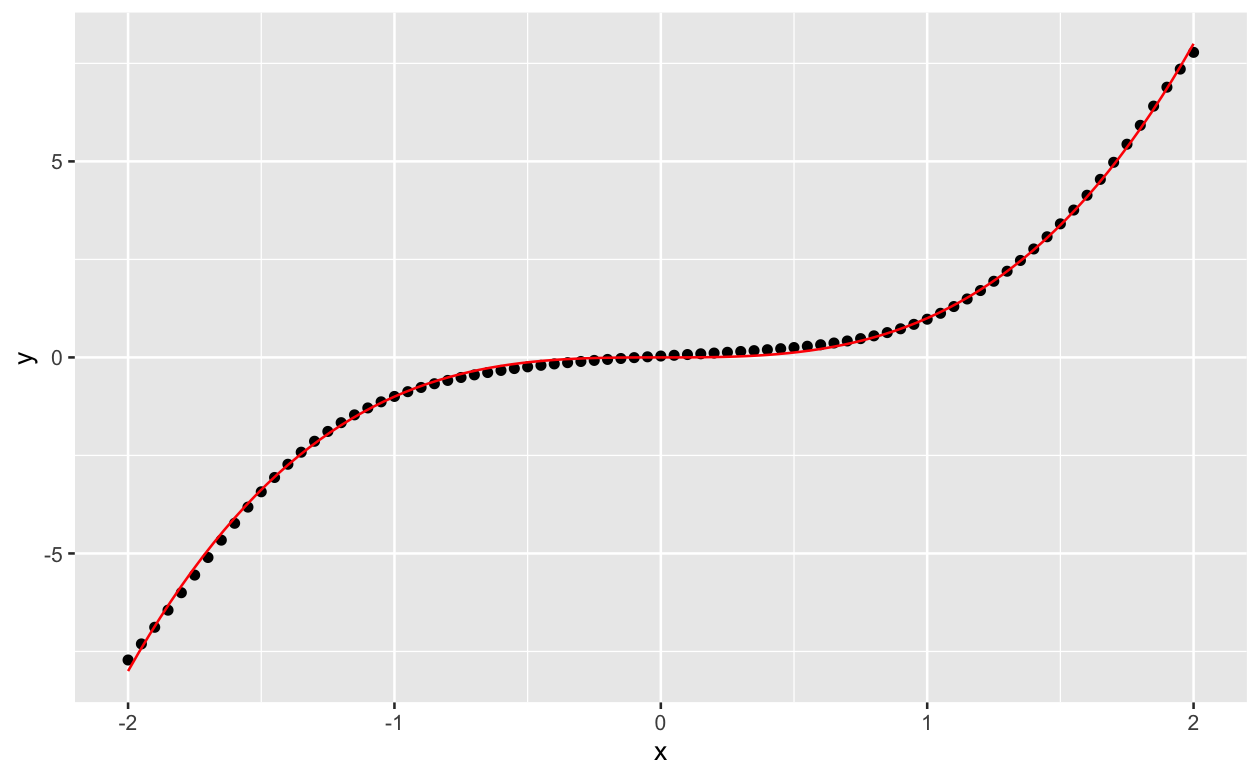
\includegraphics[width=0.9\textwidth]{img/img1.jpg}
        \caption{}
    \end{center}
\end{figure}

\section{Learning Keras}
In this assignment we will fit a neural network for classifying images. We will use Keras, which is an extensive deep learning package in Python. Keras can be used in R through the keras package. But first we need to install it, see the steps below.

To get started with Keras follow the tutorial at \url{https://keras.rstudio.com/articles/getting\_started.html}.

The documentationt to the fit function is availible at: \url{https://keras.rstudio.com/reference/fit.keras.engine}. training.Model.html. Look at the documentation and answer the following questions:

- Explain what a batch size is.
- Explain what an epoch is.
- Explain why the shuffle argument is default set to true, i.e. why do you want to shuffle? Can you think of example’s when shuffling is a bad idea?

\subsection{Batch Size}
Is the number of samples that will be propagated through the network per gradient update, that is to say in one forward/backward pass. Some of the advantages of using a batch size smaller than the number of all samples are that it requires less memory and that the training process is usually faster because we update the weights after each propagation. A disadvantage of using a batch size smaller than the number of samples is that the smaller the batch the less accurate the estimate of the gradient will be. In general we have
\begin{itemize}
    \item  \textbf{Batch Gradient Descent}. Batch Size = Size of Training Set
    \item \textbf{Stochastic Gradient Descent}. Batch Size = 1
    \item \textbf{Mini-Batch Gradient Descent}. 1 < Batch Size < Size of Training Set. Popular batch sizes include 32, 64, and 128 samples.
\end{itemize}

\subsection{Epoch}
In general, one epoch means that each sample in the training dataset has had an opportunity to update the internal model parameters, an epoch is comprised of one or more batches. A way to understand it is the following: we have a first for-loop over the number of epochs, in each loop we will a nested for-loop that iterates over each batch of sample.

In keras, the epoch parameter defines the number times that the learning algorithm will work through the entire training dataset.

\subsection{Shuffle}
This argument is a boolean that determines whether to shuffle the trining data before each epoch. The reason to set it by default is that we want the model to understand all inputs equally. For example, if the data is ordered by class, then the training result will be a bad one because the model will have a higher accuracy for the last class it trains than the first one.

Another reason why shuffle is true by default is that the objective function might have numerous minima, and therefore gradient descent algorithms are susceptible to becoming "stuck" in those minima. This is likely to occur if the set of observations is unchanged over all training iterations. Shuffling observations might help the solver to "bounce" out of a local minimum.

For the Batch Gradient Descent process (Batch Size = Size of Training Set) shuffling is unnecessary.


\section{Fitting a Model in keras}

Now we'll fit a feed-forward neural network to the dataset \textit{dataset\_fashion\_mnist()}. For the following part python was used.

\begin{python}
import keras
from keras.models import Sequential
from keras.layers import Dense, Dropout, Flatten, Conv2D, MaxPooling2D
from keras.datasets import fashion_mnist

from matplotlib import pyplot as plt

# Loading fashion_mnist dataset
fashion_mnist = keras.datasets.fashion_mnist
(train, test = fashion_mnist.load_data()
(train_images, train_labels) = train
(test_images, test_labels) = test

# Turning pixel values to values in the interval $[0,1]$
train_images = train_images / 255.0
test_images = test_images / 255.0

# Reshaping
train_images = train_images.reshape(-1,28,28,1)
train_images = train_images.astype('float32')
test_images = test_images.reshape(-1,28,28,1)
test_images = test_images.astype('float32')

# Neural net architecture
model = Sequential()

# Convolutional and max pooling layers since we are dealing with images
model.add(Conv2D(filters=64, kernel_size=2,
                 padding='same', activation='relu',
                 input_shape=(28,28,1)))
model.add(MaxPooling2D(pool_size=2))
# Dropout to deal with overfitting
model.add(Dropout(0.25))

# Repeat convolutional - max pooling - dropout
model.add(Conv2D(filters=32, kernel_size=2,
                 padding='same', activation='relu'))
model.add(MaxPooling2D(pool_size=2))
model.add(Dropout(0.25))

# Flattening
model.add(Flatten())

# Dense layer with 128 hidden units and relu activation
model.add(Dense(128, activation='relu'))

# Droput to deal with overfitting
model.add(Dropout(0.5))

# Output layer
model.add(Dense(10, activation='softmax'))

# Compiling model
model.compile(loss = 'sparse_categorical_crossentropy',
              optimizer = keras.optimizers.adam(),
              metrics = ['accuracy'])

# Training
model.fit(train_images, train_labels, epochs=10, validation_split=0.2)

# Evaluating
test_loss, test_acc = model.evaluate(test_images,  test_labels, verbose=2)
# Test error = 0.914

# Plotting validation curve
history = model.history
plt.plot(history.history['accuracy'])
plt.plot(history.history['val_accuracy'])
plt.title('model accuracy')
plt.ylabel('accuracy')
plt.xlabel('epoch')
plt.legend(['train', 'val'], loc='upper left')
plt.show()
\end{python}

The test error was $.914$ and the validation curve is given in the following figure:
\begin{figure}[H]
    \begin{center}
        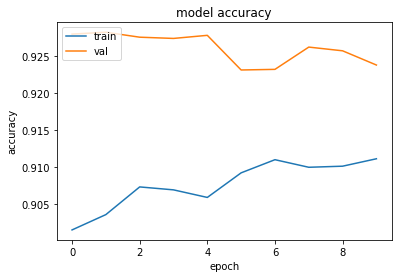
\includegraphics[width=0.8\textwidth]{img/img2.jpg}
        \caption{Validation curve}
    \end{center}
\end{figure}


\end{document}
